\documentclass[tikz,border=2pt]{standalone}
\usepackage{amsmath}
\usepackage{pgfplots}
\pgfplotsset{compat=1.18}

\begin{document}
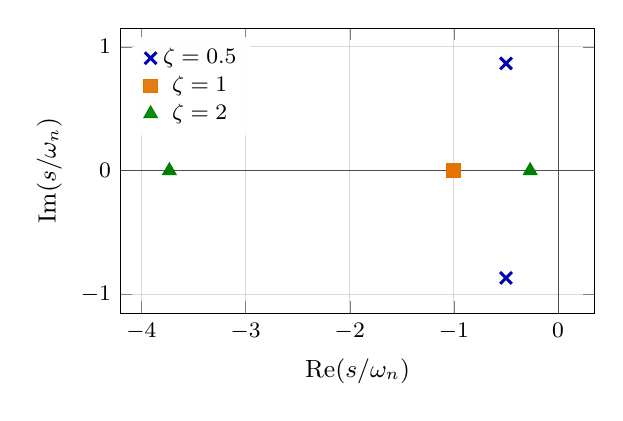
\begin{tikzpicture}
\begin{axis}[
    width=7.6cm,
    height=5.2cm,
    xmin=-4.2,
    xmax=0.35,
    ymin=-1.15,
    ymax=1.15,
    xtick={-4,-3,-2,-1,0},
    ytick={-1,0,1},
    xlabel={$\operatorname{Re}(s/\omega_n)$},
    ylabel={$\operatorname{Im}(s/\omega_n)$},
    grid=both,
    major grid style={draw=gray!30},
    tick label style={font=\footnotesize},
    label style={font=\small},
    legend style={
        at={(0.03,0.97)},
        anchor=north west,
        draw=none,
        fill=white,
        fill opacity=0.92,
        text opacity=1,
        font=\footnotesize,
        row sep=-1pt
    },
    clip=false
]
\addplot[black!70,thin,forget plot] coordinates {(-4.2,0) (0.35,0)};
\addplot[black!70,thin,forget plot] coordinates {(0,-1.15) (0,1.15)};

\addplot[
    only marks,
    mark=x,
    mark size=3pt,
    line width=1.1pt,
    blue!70!black
] coordinates {(-0.5,0.8660254) (-0.5,-0.8660254)};
\addlegendentry{$\zeta=0.5$}

\addplot[
    only marks,
    mark=square*,
    mark size=2.5pt,
    orange!90!black
] coordinates {(-1,0)};
\addlegendentry{$\zeta=1$}

\addplot[
    only marks,
    mark=triangle*,
    mark size=2.8pt,
    green!50!black
] coordinates {(-3.7320508,0) (-0.2679492,0)};
\addlegendentry{$\zeta=2$}
\end{axis}
\end{tikzpicture}
\end{document}
